\documentclass[border=0.5cm]{standalone}
 
% Packages
\usepackage[RPvoltages]{circuitikz}
\usepackage{pgfplots}
 
\begin{document}
 
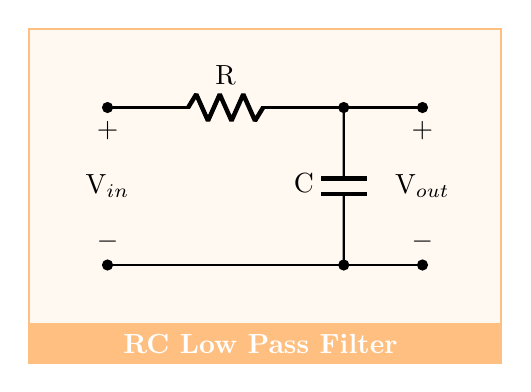
\begin{tikzpicture}[american,thick]
 
% Change components size
\ctikzset{
    resistors/scale=0.8,
    capacitors/scale=0.7,
}
 
% Orange boxes
\draw
[
    fill=orange!5,
    draw=orange!50
] (-1,-0.75) rectangle(5,3);
 
\node
[
    align=center,
    minimum width=6cm,
    fill=orange!50,
    text=white,
    draw=orange!50
] at (2,-1){\textbf{RC Low Pass Filter} };
 
% Circuit code
\draw (0,0) to[short,*-*] ++ (4,0);
\draw (0,2) to[R=R,*-] ++ (3,0) coordinate(a);
\draw (a) to[short,-*] ++ (1,0);
\draw (a) to[C,l_=C,*-*] ++(0,-2);
 
% Voltage labels
\draw (0,2) to[open,v=V$_{in}$] ++(0,-2);
\draw (4,2) to[open,v=V$_{out}$] ++(0,-2);
 
\end{tikzpicture}

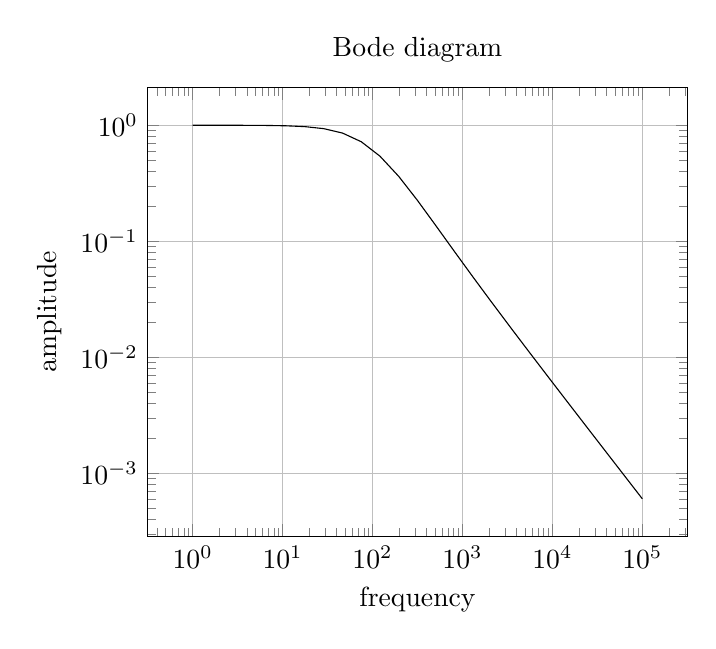
\begin{tikzpicture}
\begin{loglogaxis}[
title=Bode diagram,
xlabel={frequency},
ylabel={amplitude},
grid=major
                    ]
\addplot[domain=1:100000]  {(60*x+10000)/(x*x + 60*x+10000)};
\end{loglogaxis}
\end{tikzpicture}

\end{document}